\documentclass[12pt,a4paper,hidelinks]{article}

\usepackage{ulem}
\usepackage{incgraph}
\usepackage{tikz}
\usepackage{hyperref}

\newcommand{\leftcoordinate}{-15cm}
\usetikzlibrary{mindmap,shadows,calendar,fadings}
\tikzset{todo/.append style={annotation,above,concept color=white,draw=black,text width=2cm,align=center}}
\hypersetup{
    colorlinks=false,
    linkcolor=black,
    filecolor=magenta,      
    urlcolor=cyan,
}

\begin{document}
\begin{inctext}
    \begin{tikzpicture}
        \pgfdeclarelayer{background}
        \pgfdeclarelayer{foreground}
        \pgfsetlayers{background,main,foreground}
        % ------------------------ declare mindmap ------------------------ %
        \begin{scope}[
                mindmap,
                grow cyclic,
                concept color=red!60!green!100!blue!20,
                every node/.append style={concept,circular drop shadow},
                %level 1/.append style={sibling angle=360/6}
                every child/.append style={text width=4cm, level distance=7cm,font=\fontsize{10pt}{12pt}}
            ]
            \node[root concept, fill=white](latex){
                \href{../tex.pdf}{\LaTeX}
            }
            child{
                    node(pgf){
                            PGF
                        }
                    child{
                            node(pgfm){
                                    \href{../../../../../Documents/pgfmanual.pdf}{PGF Mannual}
                                }
                        }
                    child{
                            node(tikz){
                                    \href{run:./pgf/tikz/tikz.pdf}{Tikz}
                                }
                        }
                }
            child{
                    node(latexg){
                            \href{../../../../Documents/latex_beginners_guide.pdf}{\LaTeX\\Beginners Guide}
                        }
                }
            child{
                    node{
                            \href{https://www.overleaf.com/learn/latex/Code_Highlighting_with_minted}{Code Highlighing with Minted}
                        }
                    child{
                            node(codel){
                                    \href{https://www.overleaf.com/learn/latex/Code_listing}{Code Listing}
                                }
                        }
                }
            child[concept color=gray]{
                    node{
                            \href{https://tex.stackexchange.com/questions/606857/how-to-make-a-href-link-open-multiple-pages}{href Multiple Pages}
                        }
                }
            child{
                    node{
                            \href{https://tex.stackexchange.com/questions/512420/auto-adjust-the-width-of-tcolorbox-right-hand-side}{tcb\\listing}
                        }
                }
            child{
                    node{
                            \href{https://www.dickimaw-books.com/latex/novices/html/auxiliary.html}{Auxiliary Files}
                        }
                    child{
                            node{
                                    \href{https://www.dickimaw-books.com/latex/novices/html/crossref.html\#sec:crossref}{Cross Referencing}
                                }
                            child {
                                    node{
                                            \href{https://texfaq.org/FAQ-extref}{Referring to labels in other Documents}
                                        }
                                }
                        }
                }
            ;
        \end{scope}
        % ------------------------ background ------------------------ %
        \begin{pgfonlayer}{background}

        \end{pgfonlayer}
        % ------------------------ foreground ------------------------ %
        \begin{pgfonlayer}{foreground}
            \node[text width=1cm, text height=1cm,yshift=-1.1cm] at (latex) {
                \href{../../../mindmap.pdf}{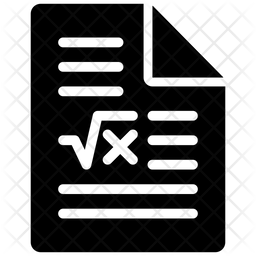
\includegraphics[width=1cm,height=1cm]{../../../image/latex.png}}
            };
            \node[text width=.5cm, text height=.5cm,yshift=-.6cm] at (pgfm) {
                
\includegraphics[width=.5cm,height=.5cm]{../../../image/book2.png}
            };
            \node[text width=1cm, text height=1cm,yshift=-1.15cm] at (latexg) {
                
\includegraphics[width=1cm,height=1cm]{../../../image/book2.png}
            };
            \node[text width=.6cm, text height=.6cm,yshift=-.5cm] at (tikz) {
                
\includegraphics[width=.6cm,height=.6cm]{../../../image/tikz.png}
            };
            \node[text width=1cm, text height=1cm,yshift=-1cm] at (codel) {
                
\includegraphics[width=1cm,height=1cm]{../../../image/star.png}
            };
        \end{pgfonlayer}
    \end{tikzpicture}
\end{inctext}
%------------------------------------------------------------ List ------------------------------------------------------------%
\newpage
\end{document}